% !TeX program = lualatex
\documentclass[DIV=12, parskip=half, fontsize=12pt, a4paper]{scrartcl}

%\usepackage[utf8]{inputenc}
%\usepackage[T1]{fontenc}    % Font-Encoding
%\usepackage{lmodern}        % LModern font
\usepackage[ngerman]{babel} % deutsche Lokalisierung
%\usepackage{graphicx}       % Einbindung von Bildern
\usepackage{pdfpages}


\usepackage{lineno}         % Nummerierung der Zeilen
%\usepackage{csquotes}       % bessere Anführungszeichen
%\usepackage{eurosym}        % Euro-Zeichen setzen
%\usepackage[normalem]{ulem} % Durchstreichen von Text-Passagen
%\usepackage[shortlabels]{enumitem} % bessere Aufzählungen mit Kurzschreibweise der Labels

\usepackage{pdfpages}       % erlaubt das Einbinden von Seiten anderer PDF-Dateien



\title{Antrag zur Neufassung der Fachschaftswahlordnung (FSWO)}
\author{Fachschaftenkonferenz}
\date{\today}

\begin{document}
  \maketitle
  Das SP möge auf Vorschlag der Fachschaftenkonferenz beschließen:

  \begin{linenumbers}
    Die Wahlordnung für die Wahlen der Fachschaftsvertretungen und Fachschaftsräte der Studierendenschaft der Rheinischen Friedrich-Wilhelms-Universität Bonn vom 16. Mai 2017 wird durch die beigefügte Wahlordnung geändert und neugefasst.

    Das  SP-Präsidium und das Fachschaftenkolletiv  werden  damit  beauftragt,  diesen Beschluss unverzüglich auszufertigen und die neugefasste Wahlordnung zur Veröffentlichung durch die Öffentlichkeitsbeauftragte zu bringen.
  \end{linenumbers}

  \vspace{1em}
  \textit{Ausgefertigt aufgrund des Beschlusses der Fachschaftenkonferenz am 9. November 2020.}

  Bonn, den \today \\
  Christoph Liedel \\
  {\scriptsize Vorsitzender des Fachschaftenkollektivs, Fachschaftenreferent}

  \clearpage
  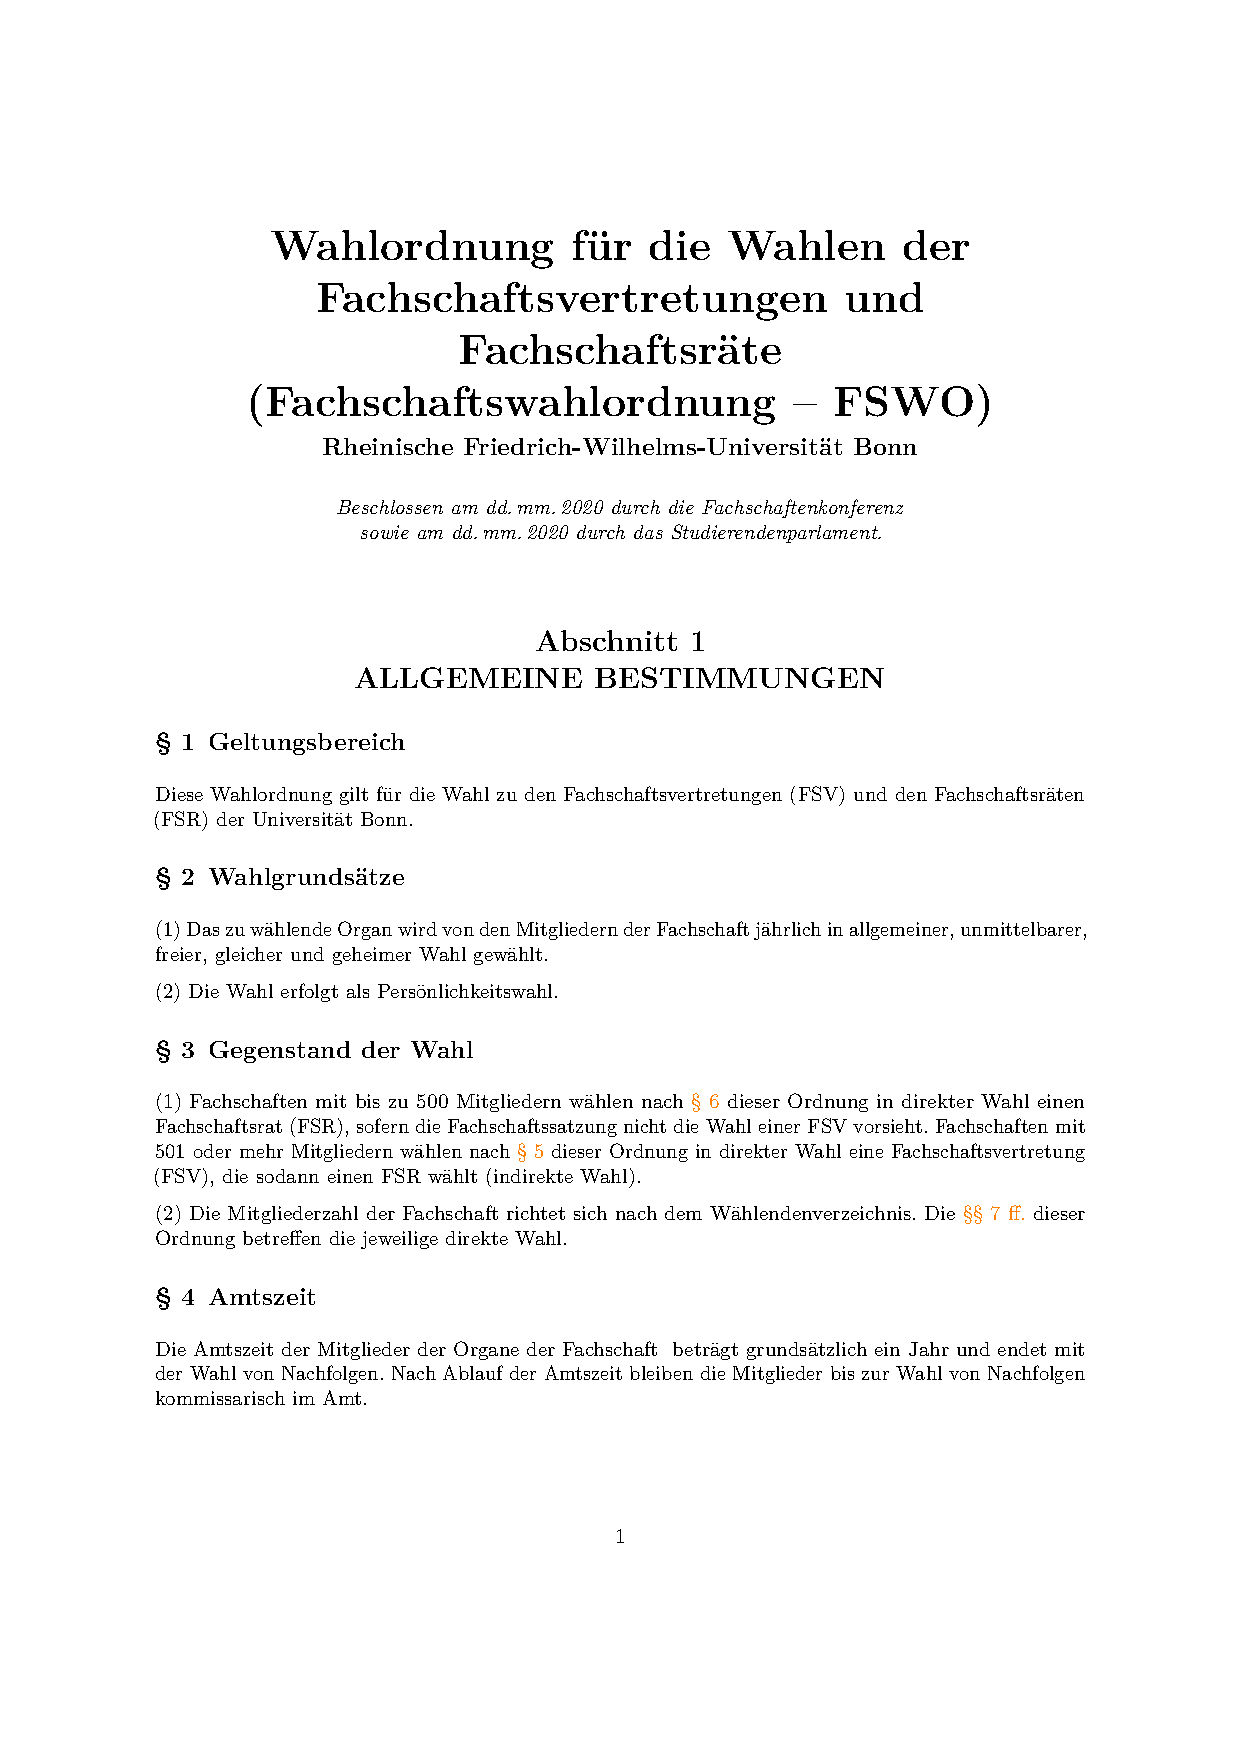
\includepdf[pages=-]{FSWO-Entwurf-ohne-Anmerkungen}
\end{document}
